\begin{titlepage}

\newgeometry{margin=.5in}     

\begin{picture}(0,0)
    \put(-100,-850){\color{mygray}\rule{16cm}{60cm}}
    %\put(-242,-100){\color{myblue}\rule{\paperwidth}{3cm}}
    \put(-20,-140){\color{black}\Huge\textbf{Documentación del Sistema}}
    \put(-20,-170){\color{black}\Huge\textbf{de Gestión del POETY}}

    \put(-20,-480){\color{black} \Large \textbf{Estatus del documento}: \hspace{1cm} En proceso}
    \put(-20,-500){\color{black} \Large \textbf{Versión}: \hspace{5cm} 0.1}
    \put(-20,-520){\color{black} \Large \textbf{Fecha de entrega}: \hspace{2.5cm} \today}
    \put(-20,-540){\color{black} \Large \textbf{Autores}: \hspace{5cm} }

    \put(-20,-750){\color{black} \small \textbf{Ciudad Universitaria. Circuito exterior s/n anexo al Jardín Botánico Exterior.}}
     \put(-20,-760){\color{black} \small \textbf{UNAM 04510. Ciudad de México. Apartado Postal 70-275.}}

\end{picture}

\vskip3.5cm

\begin{minipage}[t]{0.6\textwidth}
\large
\vspace{1cm}
\subsubsection*{Resumen:}

Se presenta la metodología del diseño de un sistema que tiene por objetivo diseñar, desarrollar e implementar un sistema de gestión para el ordenamiento ecológico del territorio del estado de Yucatán (Sistema) que funcione como un sistema de información geográfica para la puesta en marcha de la actualización del POETY, para el manejo y análisis  de información que facilite la gobernanza colaborativa en el proceso de ordenamiento ecológico en la entidad y su articulación con otros instrumentos de planeación pertinentes.
\end{minipage}%
\hfill
\begin{minipage}[t]{0.25\textwidth} 
  
\includegraphics[width=47mm]{images/UNAM}\vspace{2cm}
  
\includegraphics[width=42mm]{images/ie_logo}\vspace{2cm}
  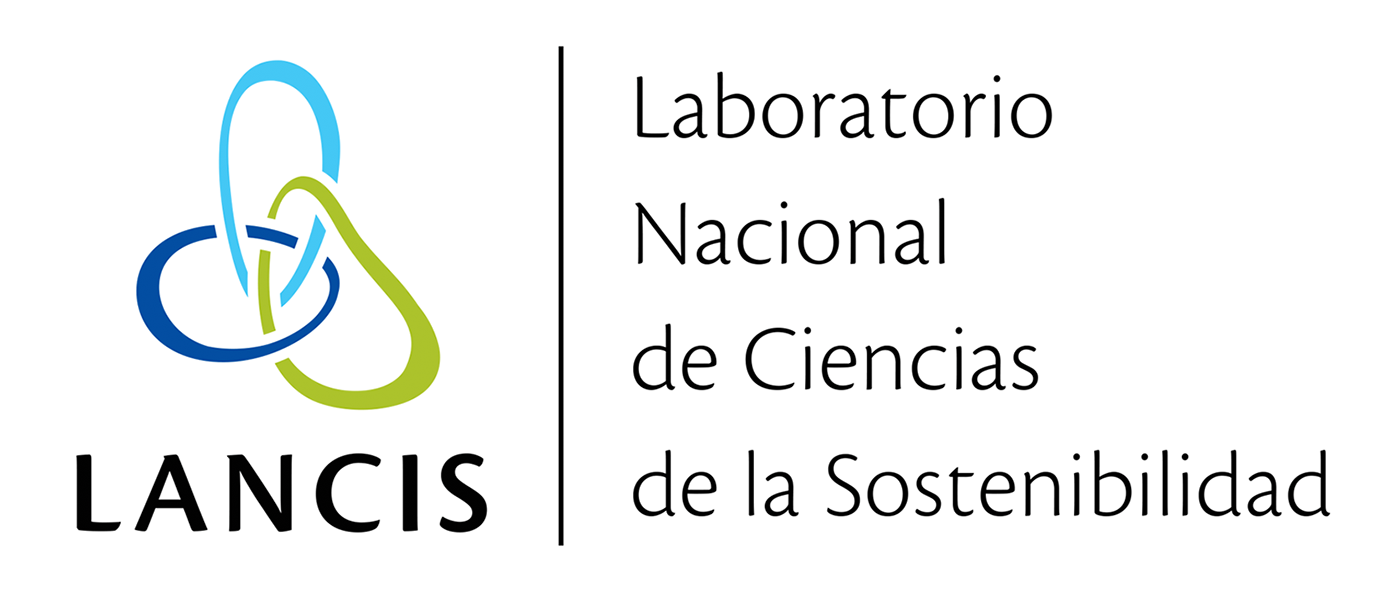
\includegraphics[width=60mm]{images/lancis_logo}\vspace{2cm}
  
\includegraphics[width=52mm]{images/yucatan_logo}%
\end{minipage}

\end{titlepage}

\pagebreak

\restoregeometry